\documentclass[final]{beamer}
\usepackage{eulervm,verbatim}          
\usepackage[scaled]{helvet}
\usepackage[most]{tcolorbox}
\setbeamercolor{frametitle}{fg=black,bg=white} % Colors of the block titles
\setbeamertemplate{caption}{\raggedright\insertcaption\par}
\setbeamertemplate{caption}{\raggedright\insertcaption\par}
\definecolor{darkcerulean}{rgb}{0.03, 0.27, 0.49}
\newcommand{\citesmall}[1]{[{\color{darkcerulean}\begin{small} \textbf{#1} \end{small}}]}
\setbeamertemplate{footline}[frame number]
\DeclareMathOperator*{\argmin}{arg\,min}
\usepackage{graphicx}  % Required for including images
\usepackage{bbm}
\usepackage{booktabs} % Top and bottom rules for tables
\definecolor{burgundy}{rgb}{0.5, 0.0, 0.13}
\newcommand{\highlight}[1]{{\color{burgundy} \textbf{#1}}}
\usepackage{hyperref}
\hypersetup{
    colorlinks=true,
    linkcolor=blue,
    filecolor=magenta,      
    urlcolor=magenta,
    pdftitle={CSE6740-Lecture 1},
    pdfauthor={Nisha Chandramoorthy},
    pdflang={en-US}
}



%----------------------------------------------------------------------------------------
%	TITLE SECTION 
%----------------------------------------------------------------------------------------
\title{\begin{huge}{CSE 6740 A/ISyE 6740: Computational Data Analysis: Introductory lecture}\end{huge}} % Poster title


\author{Nisha Chandramoorthy} % Author(s)


%----------------------------------------------------------------------------------------

\begin{document}

\frame{\titlepage}

%----------------------------------------------------------------------------------------
%	OBJECTIVES
%----------------------------------------------------------------------------------------
\begin{frame}{Course logistics}
\begin{itemize}
	\item Instructor: Nisha Chandramoorthy. 
	\pause
	\item Interested in teaching and learning about foundations of machine learning
	\pause
	\item 6 TAs: Akpevwe Ojameruaye, Atharva Ketkar, Chengrui Li, Darryl Jacob, Mithilesh Vaidya, and Yusen Su 
	\pause
	\item Lectures: TR 12:30-1:45 pm. OH: 30 minutes after. Location: East Architecture 123.
	\pause
	\item Grade: 4 homeworks (30\%), 2 midterms (30\%), final project (40\%)
	\pause
\item \href{https://canvas.gatech.edu}{Canvas} (see syllabus), \href{https://www.gradescope.com/courses/578036}{gradescope}, \href{https://piazza.com/gatech/fall2023/cse6740a/info}{Piazza}, \href{https://github.com/ni-sha-c/CSE-6740-Fall23}{Github}
\end{itemize}
\end{frame}

\begin{frame}{Machine learning and data mining: what are they?}
\begin{itemize}
	\item ``Automated detection of meaningful patterns in data'' - Shalev-Shwartz and Ben-David.
	\pause
	\item  Goal in this class: understand the foundations (``why''s and ``how''s) of ML
	\pause
	\item ML = Compute + data
	\pause
	\item Compute: Optimization, representation/models
	\pause
	\item Data: distributions, features/compression, statistics
\end{itemize}
\end{frame}
\begin{frame}{Categorizations of learning}
	\begin{itemize}
		\item Supervised, unsupervised, self-supervised, semi-supervised 
		\pause
	\item Supervised: using \emph{experience} (training data) to learn  
	\pause
	\item Unsupervised: using \emph{data} to identify patterns, match distributions?
	\pause
	\item Mode of learning and testing are different
	\pause
	\item You sample peaches across several grocery stores in Atlanta. Now you are given a new peach of unknown origins. Can you tell if it would taste good?  
	\end{itemize}
	
\end{frame}
\begin{frame}{Supervised, unsupervised, in-between, semi-supervised, self-supervised...}
	\begin{figure}
		\centering
		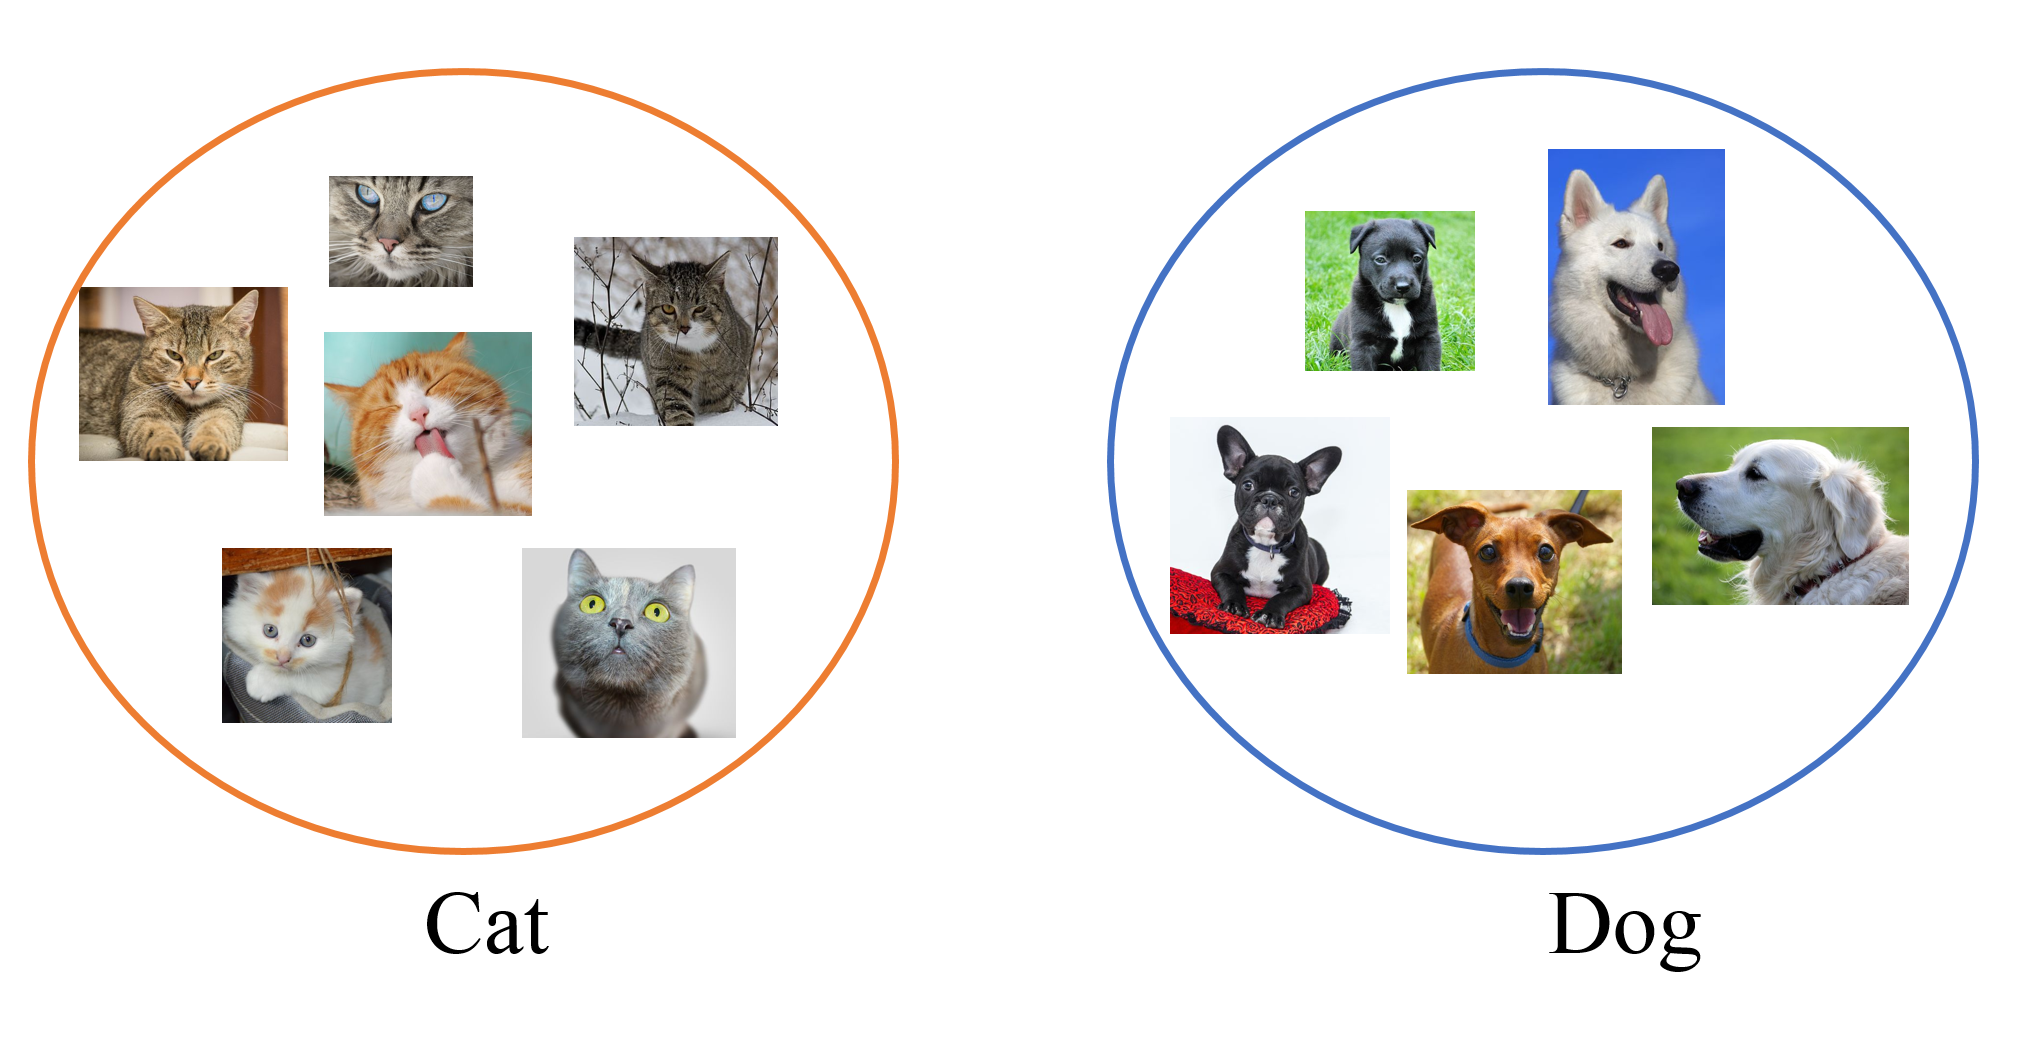
\includegraphics[width=0.4\textwidth]{clustering.png}
		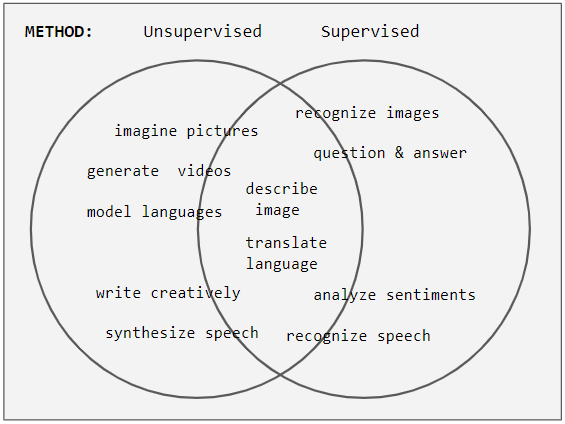
\includegraphics[width=0.5\textwidth]{supervisedVsUnsupervised.png}
	\end{figure}
	\begin{itemize}
		\item Many modern tasks require both modes of learning
		\pause
		\item 5 * 9 = -4, 4 + 10 = 6, 8 * 7 = 1, 5 + 2 = -3, (3 * 5) + 6 = ?
		\pause
		\item You are feeling sleepy this afternoon. You order a ...
		\pause
		\item New research frontier for theory: understand how and why large ML models work the way they do?
	\end{itemize}

\end{frame}
\begin{frame}{Models/representations, algorithms, statistical principles}
	\begin{itemize}
		\item how to make and test conjectures about how large language models (LLMs) learn?
		\pause
		\item ``how to train them better (more efficiently)'' -- number of practical questions perhaps benefit from theory
		\pause 
		\item AI safety, fair and ethical ethical use, combining with other domain knowledge (e.g., physics, chemistry etc).... and many more!
		\pause 
		\item Perhaps biggest contribution advance to LLMs: transformers and their training.
	\end{itemize}
\end{frame}
\begin{frame}{(partial) History - trace back from transformers (source:Wikipedia)}
	\begin{itemize}
		\item Transformer architecture: 2017, Google Brain [Vaswani et al]
		\item Deep learning, unsupervised learning 2010s (e.g., GANs 2014)...
		\item ImageNet: 2009, Fei Fei Li 
		\item Long-short term memory (LSTM) architecture: 1997, [Hochreiter and Schmidhuber]
		\item Convolutional NNs: (inspired from) 1979 work by [Fukushima];  Recurrent neural networks: 1982 [Hopfield]
		\item ...
		\item Automatic Differentiation: 1970 [Linnainmaa]
		\item ...
		\item First neural networks: 1950s [Minsky and others]
	\end{itemize}
\end{frame}
\begin{frame}{Supervised learning framework}
	\begin{itemize}
		\item Distribution $\mathcal{D}$ over the joint distribution of random variables $Z = (X, Y)$, where $X$ is an input and $Y$ is a label/output.
		\pause
	\item Labeled training data, $S = \{z_i = (x_i, y_i)\}, 1\leq i \leq m.$ Generally iid from $\mathcal{D}^m.$
		\pause
		\item Learner's output: predicted function or hypothesis, a transformation $h$ from $X$ to $Y$.
		\pause
	\item Loss function, measure of risk:  $\ell(z, h) \in \mathbb{R}$. e.g., $\ell(z, h) =  \mathbbm{1}_{h(x) \neq y}.$ (classification)
	\pause
	\item Generalization error or risk: 
		$$R(h) = E_{z\sim \mathcal{D}} \ell(z, h)$$
	\end{itemize}
\end{frame}
\begin{frame}{Empirical Risk Minimization}
	\begin{itemize}
		\item Take classifier $h$, $R(h) = \mathcal{D}(\{z: h(x) \neq y\}).$
		\pause
		\item When you have finite amount of data, empirical risk or training loss
		$$ \hat{R}_S(h) = \dfrac{1}{m} \sum_{z \in S} \ell(z,h) = \dfrac{|\{z \in S: h(x) \neq y\}|}{m}.$$
		\pause
	\item ERM: find $h$ that minimizes $\hat{R}_S(h).$
	\pause
	\item Theory of supervised learning suggests that ERM leads to small generalization error with high probability
	\pause
	\item Now we will prove this result formally. 
	\pause
\item Next time: Linear models.
\end{itemize}
\end{frame}
\begin{frame}{Finite hypothesis classes}
	\begin{itemize}
		\item ERM rules can lead to bad generalization
		\pause
		\item Why? Overfitting
		\pause
		\item Example
		\pause
		\item One way to reduce overfitting: inductive bias. Choose $\mathcal{H}$ based on prior knowledge.
		\pause 
		\item Later: when does memorization of training data lead to good generalization?
		\pause
	\item Now: simple case of finite $\mathcal{H}$. 
	
	\end{itemize}
\end{frame}

\end{document}
